% questions.tex —— 2010 年·全国大纲卷Ⅱ·理科 · 题目内容片段（无答案）
% 由 tools/generate_projects.py 依来源总账自 2010/2010_数学真题_全国2理_试题.md 生成，勿手改（改源 MD 后重跑）


\gkpart{数学}

\begin{gktip}
\textbf{来源说明}：本题面依据固定源 PDF 两页 A3 题面逐题转录，原卷印刷页码 585–586。固定源不附答案，答案和解析均由本库独立复算。

\textbf{图形说明}：第 19 题的直三棱柱和第 20 题的电路图重绘为 TikZ/PGFPlots 矢量图。图形标记所指的 PNG 不随仓库保存。
\end{gktip}

\gkpart{一、选择题}

\begin{question}
\gkti{1}复数 $\left(\dfrac{3-i}{1+i}\right)^2=$\mbox{（　　）}

（A）$-3-4i$\quad（B）$-3+4i$\quad（C）$3-4i$\quad（D）$3+4i$

\end{question}
\begin{question}
\gkti{2}函数 $y=\dfrac{1+\ln(x-1)}2$（$x>1$）的反函数是\mbox{（　　）}

（A）$y=e^{2x+1}-1$（$x>0$）\quad（B）$y=e^{2x-1}+1$（$x>0$）

（C）$y=e^{2x+1}-1$（$x\in\mathbb R$）\quad（D）$y=e^{2x-1}+1$（$x\in\mathbb R$）

\end{question}
\begin{question}
\gkti{3}若变量 $x,y$ 满足约束条件

\nopagebreak[4]
\[
\begin{cases}
y\geq x,\\
x\geq-1,\\
3x+2y\leq5,
\end{cases}
\]

则 $z=2x+y$ 的最大值为\mbox{（　　）}

（A）$1$\quad（B）$2$\quad（C）$3$\quad（D）$4$

\end{question}
\begin{question}
\gkti{4}如果等差数列 $\{a_n\}$ 中，$a_3+a_4+a_5=12$，那么 $a_1+a_2+\cdots+a_7=$\mbox{（　　）}

（A）$14$\quad（B）$21$\quad（C）$28$\quad（D）$35$

\end{question}
\begin{question}
\gkti{5}不等式 $\dfrac{x^2-x-6}{x-1}>0$ 的解集为\mbox{（　　）}

（A）$\{x\mid x<-2\text{ \text{或} }x>3\}$\quad（B）$\{x\mid x<-2\text{ \text{或} }1<x<3\}$

（C）$\{x\mid-2<x<1\text{ \text{或} }x>3\}$\quad（D）$\{x\mid-2<x<1\text{ \text{或} }1<x<3\}$

\end{question}
\begin{question}
\gkti{6}将标号为 $1,2,3,4,5,6$ 的 $6$ 张卡片放入 $3$ 个不同的信封中，若每个信封放 $2$ 张，其中标号为 $1,2$ 的卡片放入同一信封，则不同的放法共有\mbox{（　　）}

（A）$12$ 种\quad（B）$18$ 种\quad（C）$36$ 种\quad（D）$54$ 种

\end{question}
\begin{question}
\gkti{7}为了得到函数 $y=\sin\left(2x-\dfrac\pi3\right)$ 的图象，只需把函数 $y=\sin\left(2x+\dfrac\pi6\right)$ 的图象\mbox{（　　）}

（A）向左平移 $\dfrac\pi4$ 个长度单位\quad（B）向右平移 $\dfrac\pi4$ 个长度单位

（C）向左平移 $\dfrac\pi2$ 个长度单位\quad（D）向右平移 $\dfrac\pi2$ 个长度单位

\end{question}
\begin{question}
\gkti{8}$\triangle ABC$ 中，点 $D$ 在边 $AB$ 上，$CD$ 平分 $\angle ACB$。若 $\overrightarrow{CB}=\boldsymbol a$，$\overrightarrow{CA}=\boldsymbol b$，$|\boldsymbol a|=1$，$|\boldsymbol b|=2$，则 $\overrightarrow{CD}=$\mbox{（　　）}

（A）$\dfrac13\boldsymbol a+\dfrac23\boldsymbol b$\quad（B）$\dfrac23\boldsymbol a+\dfrac13\boldsymbol b$\quad（C）$\dfrac35\boldsymbol a+\dfrac45\boldsymbol b$\quad（D）$\dfrac45\boldsymbol a+\dfrac35\boldsymbol b$

\end{question}
\begin{question}
\gkti{9}已知正四棱锥 $S-ABCD$ 中，$SA=2\sqrt3$，那么当该棱锥的体积最大时，它的高为\mbox{（　　）}

（A）$1$\quad（B）$\sqrt3$\quad（C）$2$\quad（D）$3$

\end{question}
\begin{question}
\gkti{10}若曲线 $y=x^{-\frac12}$ 在点 $\left(a,a^{-\frac12}\right)$ 处的切线与两个坐标轴围成的三角形面积为 $18$，则 $a=$\mbox{（　　）}

（A）$64$\quad（B）$32$\quad（C）$16$\quad（D）$8$

\end{question}
\begin{question}
\gkti{11}与正方体 $ABCD-A_1B_1C_1D_1$ 的三条棱 $AB\text{、}CC_1\text{、}A_1D_1$ 所在直线的距离相等的点\mbox{（　　）}

（A）有且只有 $1$ 个\quad（B）有且只有 $2$ 个\quad（C）有且只有 $3$ 个\quad（D）有无数个

\end{question}
\begin{question}
\gkti{12}已知椭圆 $C:\dfrac{x^2}{a^2}+\dfrac{y^2}{b^2}=1$（$a>b>0$）的离心率为 $\dfrac{\sqrt3}{2}$，过右焦点 $F$ 且斜率为 $k$（$k>0$）的直线与 $C$ 相交于 $A\text{、}B$ 两点。若 $\overrightarrow{AF}=3\overrightarrow{FB}$，则 $k=$\mbox{（　　）}

（A）$1$\quad（B）$\sqrt2$\quad（C）$\sqrt3$\quad（D）$2$

\end{question}
\gkpart{二、填空题}

\begin{question}
\gkti{13}已知 $\alpha$ 是第二象限的角，$\tan(\pi+2\alpha)=-\dfrac43$，则 $\tan\alpha=$\gkblank{}。

\end{question}
\begin{question}
\gkti{14}若 $\left(x-\dfrac ax\right)^9$ 的展开式中 $x^3$ 的系数是 $-84$，则 $a=$\gkblank{}。

\end{question}
\begin{question}
\gkti{15}已知抛物线 $C:y^2=2px$（$p>0$）的准线为 $l$，过 $M(1,0)$ 且斜率为 $\sqrt3$ 的直线与 $l$ 相交于点 $A$，与 $C$ 的一个交点为 $B$。若 $\overrightarrow{AM}=\overrightarrow{MB}$，则 $p=$\gkblank{}。

\end{question}
\begin{question}
\gkti{16}已知球 $O$ 的半径为 $4$，圆 $M$ 与圆 $N$ 为该球的两个小圆，$AB$ 为圆 $M$ 与圆 $N$ 的公共弦，$AB=4$。若 $OM=ON=3$，则两圆圆心的距离 $MN=$\gkblank{}。

\end{question}
\gkpart{三、解答题}

\begin{question}
\gkti{17}$\triangle ABC$ 中，$D$ 为边 $BC$ 上的一点，$BD=33$，$\sin B=\dfrac5{13}$，$\cos\angle ADC=\dfrac35$，求 $AD$。

\end{question}
\begin{question}
\gkti{18}已知数列 $\{a_n\}$ 的前 $n$ 项和 $S_n=(n^2+n)\cdot3^n$。

（1） 求 $\displaystyle\lim_{n\to\infty}\dfrac{a_n}{S_n}$；

（2） 证明：$\displaystyle\frac{a_1}{1^2}+\frac{a_2}{2^2}+\cdots+\frac{a_n}{n^2}>3^n$。

\Needspace{0.4\textheight}
\end{question}
\begin{question}
\gkti{19}如图，直三棱柱 $ABC-A_1B_1C_1$ 中，$AC=BC$，$AA_1=AB$，$D$ 为 $BB_1$ 的中点，$E$ 为 $AB_1$ 上的一点，$AE=3EB_1$。
\nopagebreak[4]
\begin{center}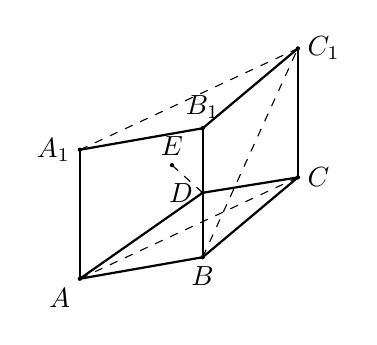
\begin{tikzpicture}[scale=.78,>=stealth]
\coordinate (A) at (0,0); \coordinate (B) at (2.0,.35);
\coordinate (C) at (3.55,1.65); \coordinate (A1) at (0,2.1);
\coordinate (B1) at (2.0,2.45); \coordinate (C1) at (3.55,3.75);
\coordinate (D) at (2.0,1.4); \coordinate (E) at (1.5,1.85);
\draw[thick] (A)--(B)--(C);
\draw[thick] (A1)--(B1)--(C1);
\draw[thick] (A)--(A1) (B)--(B1) (C)--(C1);
\draw[dashed] (A)--(C) (A1)--(C1) (B)--(C1);
\draw[thick] (A)--(D)--(C);
\draw[dashed] (D)--(E);
\fill (A) circle (1pt) node[below left] {$A$};
\fill (B) circle (1pt) node[below] {$B$};
\fill (C) circle (1pt) node[right] {$C$};
\fill (A1) circle (1pt) node[left] {$A_1$};
\fill (B1) circle (1pt) node[above] {$B_1$};
\fill (C1) circle (1pt) node[right] {$C_1$};
\fill (D) circle (1pt) node[left] {$D$};
\fill (E) circle (1pt) node[above] {$E$};
\end{tikzpicture}
\end{center}
\nopagebreak[4]
（1） 证明：$DE$ 为异面直线 $AB_1$ 与 $CD$ 的公垂线；

（2） 设异面直线 $AB_1$ 与 $CD$ 的夹角为 $45^\circ$，求二面角 $A_1-AC_1-B_1$ 的大小。

\Needspace{0.4\textheight}
\end{question}
\begin{question}
\gkti{20}如图，由 $M$ 到 $N$ 的电路中有 $4$ 个组件，分别标为 $T_1\text{、}T_2\text{、}T_3\text{、}T_4$，电流能通过 $T_1\text{、}T_2\text{、}T_3$ 的概率都是 $p$，电流能通过 $T_4$ 的概率是 $0.9$。电流能否通过各组件相互独立。已知 $T_1\text{、}T_2\text{、}T_3$ 中至少有一个能通过电流的概率为 $0.999$。
\nopagebreak[4]
\begin{center}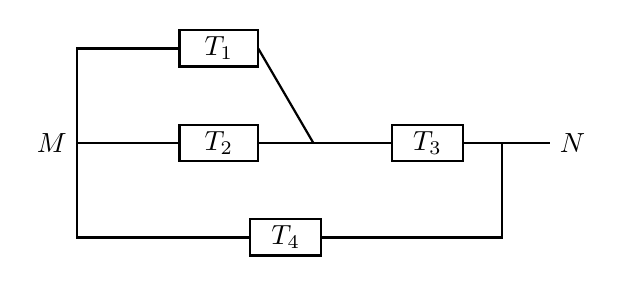
\begin{tikzpicture}[>=stealth,thick]
\coordinate (M) at (0,0); \coordinate (J) at (3,0);
\coordinate (N) at (6,0);
\draw (M)--(1.3,0);
\draw (1.3,-.23) rectangle (2.3,.23) node[pos=.5] {$T_2$};
\draw (2.3,0)--(J);
\draw (M)--(0,1.2)--(1.3,1.2);
\draw (1.3,.97) rectangle (2.3,1.43) node[pos=.5] {$T_1$};
\draw (2.3,1.2)--(J);
\draw (J)--(4.0,0);
\draw (4.0,-.23) rectangle (4.9,.23) node[pos=.5] {$T_3$};
\draw (4.9,0)--(N);
\draw (M)--(0,-1.2)--(2.2,-1.2);
\draw (2.2,-1.43) rectangle (3.1,-.97) node[pos=.5] {$T_4$};
\draw (3.1,-1.2)--(5.4,-1.2)--(5.4,0)--(N);
\node[left] at (M) {$M$}; \node[right] at (N) {$N$};
\end{tikzpicture}
\end{center}
\nopagebreak[4]
（1） 求 $p$；

（2） 求电流能在 $M$ 与 $N$ 之间通过的概率。

\end{question}
\begin{question}
\gkti{21}已知斜率为 $1$ 的直线 $l$ 与双曲线 $C:\dfrac{x^2}{a^2}-\dfrac{y^2}{b^2}=1$（$a>0,b>0$）相交于 $B\text{、}D$ 两点，且 $BD$ 的中点为 $M(1,3)$。

（1） 求 $C$ 的离心率；

（2） 设 $C$ 的右顶点为 $A$，右焦点为 $F$，$|DF|\cdot|BF|=17$，证明：过 $A\text{、}B\text{、}D$ 三点的圆与 $x$ 轴相切。

\end{question}
\begin{question}
\gkti{22}设函数 $f(x)=1-e^{-x}$。

（1） 证明：当 $x>-1$ 时，$f(x)\geq\dfrac{x}{x+1}$；

（2） 设当 $x\geq0$ 时，$f(x)\leq\dfrac{x}{ax+1}$，求 $a$ 的取值范围。

\end{question}